\chapter{Threads and Concurrency}

\section{What is a thread?}

\begin{definition}[Thread]
A \textbf{thread} is a sequence of instructions being executed, together with the state needed to
continue executing it: a program counter, register values, and a stack. A \textbf{sequential}
program has one thread; a \textbf{concurrent} program has several threads that may run at the
same time.
\end{definition}

Why use threads?
\begin{itemize}
  \item \textbf{Resource utilization}: when one thread blocks (e.g.\ waiting for disk I/O),
    another can use the CPU.
  \item \textbf{Parallelism}: on a multicore machine, threads run simultaneously and finish
    the work faster.
  \item \textbf{Responsiveness}: a GUI thread keeps responding while a worker thread computes.
  \item \textbf{Program structure}: a server handling many clients is naturally written as
    one thread per client.
\end{itemize}

Threads in the same process \emph{share} the address space: code, global variables and the heap.
Each thread has its \emph{own} stack, program counter and registers.

\begin{center}
\begin{tikzpicture}[seg/.style={draw,minimum width=3.2cm,minimum height=0.7cm}]
  \node[seg,fill=gray!15] (code) {code};
  \node[seg,below=0pt of code,fill=gray!15] (data) {global data};
  \node[seg,below=0pt of data,fill=gray!15] (heap) {heap};
  \node[seg,below=0.4cm of heap,fill=blue!10] (s1) {stack (thread 1)};
  \node[seg,below=0pt of s1,fill=green!10] (s2) {stack (thread 2)};
  \node[right=1.2cm of data,align=left,font=\small] {shared by\\all threads};
  \node[right=1.2cm of s1,align=left,font=\small] {private to\\each thread};
\end{tikzpicture}
\end{center}

\section{OS/161 thread interface}

\begin{lstlisting}[style=c]
/* kern/include/thread.h */
int  thread_fork(const char *name,          /* name for debugging */
                 struct proc *proc,         /* process the thread joins (NULL = current) */
                 void (*func)(void *, unsigned long), /* entry point */
                 void *data1, unsigned long data2);   /* args to func */
void thread_exit(void);   /* terminate the calling thread (never returns) */
void thread_yield(void);  /* voluntarily give up the CPU; stays runnable */
\end{lstlisting}

\begin{example}[Forking worker threads]
\begin{lstlisting}[style=c]
static volatile int total = 0;    /* shared! needs synchronization (Ch. 3) */

static void worker(void *p, unsigned long n) {
    (void)p;
    kprintf("worker %lu running\n", n);
    thread_exit();
}

int run_workers(void) {
    for (unsigned long i = 0; i < 4; i++) {
        int err = thread_fork("worker", NULL, worker, NULL, i);
        if (err) panic("thread_fork failed: %s\n", strerror(err));
    }
    return 0;
}
\end{lstlisting}
The order in which the workers print is \emph{non-deterministic}: it depends on the scheduler.
\end{example}

OS/161 has no \code{thread\_join}; the analogous POSIX API is \code{pthread\_create},
\code{pthread\_join}, \code{pthread\_exit}. Joining is something you build yourself with
semaphores or condition variables.

\section{Concurrent execution}

On a single core, threads take turns. Two models of concurrency:
\begin{description}
  \item[Multiprocessing / multicore] $P$ processors each run one thread at a time; up to $P$
    threads truly run in parallel.
  \item[Timesharing] Multiple threads share one processor by rapidly switching between them.
\end{description}
Real systems combine both: each core is timeshared.

\section{Context switches}

\begin{definition}[Context switch]
A \textbf{context switch} is the act of pausing the currently running thread (saving its
register state), choosing another thread to run (the \emph{scheduler}), and resuming that thread
(restoring its register state).
\end{definition}

The saved state of a thread is called its \textbf{context}. In OS/161 the context is saved on the
thread's own stack in a \code{switchframe}, and the thread structure remembers the stack
pointer.

\subsection*{Context switch in OS/161}
\begin{enumerate}
  \item The running thread calls \code{thread\_yield()} (or is preempted, or blocks).
  \item \code{thread\_yield} calls \code{thread\_switch(S\_READY, ...)}, which puts the current
    thread on the ready queue and asks the scheduler for the next thread.
  \item \code{thread\_switch} calls the assembly routine \code{switchframe\_switch}, which
    \begin{itemize}
      \item pushes the \emph{callee-saved} registers \code{s0}--\code{s8}, \code{gp}, \code{ra}
        onto the current stack (only these, since caller-saved registers were saved by the
        normal C calling convention before calling \code{thread\_switch}),
      \item saves the stack pointer into the old thread's structure,
      \item loads the new thread's saved stack pointer,
      \item pops the new thread's registers and returns --- \emph{into the new thread}.
    \end{itemize}
\end{enumerate}

\begin{figure}[H]
\centering
\begin{tikzpicture}[x=1cm, y=1cm, font=\small, >=Stealth]
  \node[anchor=east] at (-0.1,1.4) {thread A};
  \node[anchor=east] at (-0.1,0.4) {thread B};
  \draw[line width=5pt, blue!50] (0,1.4) -- (3,1.4);
  \draw[line width=5pt, gray!30] (4,1.4) -- (8,1.4);
  \draw[line width=5pt, gray!30] (0,0.4) -- (4,0.4);
  \draw[line width=5pt, green!50!black!50] (4,0.4) -- (8,0.4);
  \draw[line width=5pt, blue!50] (9,1.4) -- (11,1.4);
  \fill[orange!30] (3,0) rectangle (4,1.8);
  \fill[orange!30] (8,0) rectangle (9,1.8);
  \node[font=\scriptsize, align=center] at (3.5,2.2) {save A,\\restore B};
  \node[font=\scriptsize, align=center] at (8.5,2.2) {save B,\\restore A};
  \node[font=\scriptsize] at (1.5,1.75) {running};
  \node[font=\scriptsize] at (6,1.75) {ready};
  \node[font=\scriptsize] at (6,0.05) {running};
  \draw[->] (0,-0.3) -- (11.3,-0.3) node[right, font=\scriptsize]{time};
\end{tikzpicture}
\caption{Two context switches on one CPU. During each switch (shaded) the
kernel saves the outgoing thread's callee-saved registers in a
\code{switchframe} and restores the incoming thread's.}
\end{figure}

\begin{lstlisting}[style=mips]
# simplified switchframe_switch(a0 = &old->t_context, a1 = &new->t_context)
switchframe_switch:
    addi sp, sp, -40        # allocate stack space for 10 registers
    sw   ra, 36(sp)
    sw   gp, 32(sp)
    sw   s8, 28(sp)
    sw   s6, 24(sp)
    # ... s5..s0 ...
    sw   sp, 0(a0)          # old thread: remember its stack pointer
    lw   sp, 0(a1)          # new thread: switch to its stack
    nop                     # load delay slot
    lw   s0, 0(sp)
    # ... restore s1..s8, gp, ra ...
    j    ra                 # return into the NEW thread
    addi sp, sp, 40         # (delay slot) pop the frame
\end{lstlisting}

\begin{important}[Why only callee-saved registers?]
\code{switchframe\_switch} is called like a normal function. By the MIPS calling convention the
caller (\code{thread\_switch}) has already saved any caller-saved (temporary) registers it needs.
So the switch code only has to preserve the callee-saved ones. This is different from an
interrupt (Ch.~4), where \emph{all} registers must be saved in a trapframe because the
interrupted code did not expect to be interrupted.
\end{important}

\section{Thread states}

\begin{center}
\begin{tikzpicture}[node distance=3cm,state/.style={draw,rounded corners,minimum width=1.9cm,minimum height=0.8cm}]
  \node[state] (ready) {ready};
  \node[state,right=of ready] (run) {running};
  \node[state,below=1.6cm of $(ready)!0.5!(run)$] (blk) {blocked};
  \draw[-{Stealth},bend left=20] (ready) to node[above,font=\small]{dispatch} (run);
  \draw[-{Stealth},bend left=20] (run) to node[below,font=\small,align=center]{yield /\\preempt} (ready);
  \draw[-{Stealth}] (run) to node[right,font=\small]{sleep (wait)} (blk);
  \draw[-{Stealth}] (blk) to node[left,font=\small]{wakeup} (ready);
\end{tikzpicture}
\end{center}

\begin{description}
  \item[Running] currently executing on a CPU.
  \item[Ready] could run, waiting for a CPU; kept on the \textbf{ready queue}.
  \item[Blocked] waiting for something (a lock, I/O, a semaphore); kept on a \textbf{wait
    channel} (\code{struct wchan} in OS/161). Only another thread or an interrupt handler can
    wake it, moving it back to ready.
\end{description}
In OS/161 a thread blocks with \code{wchan\_sleep(wc, lock)} and is woken with
\code{wchan\_wakeone} / \code{wchan\_wakeall}. Transitions out of running are:
\code{thread\_yield} (running $\to$ ready), \code{wchan\_sleep} (running $\to$ blocked),
\code{thread\_exit} (running $\to$ zombie/destroyed).

\section{Preemption and timesharing}

If a thread never calls \code{thread\_yield} or blocks, a cooperative system would let it hog the
CPU forever. \textbf{Preemption} forces a context switch.

\begin{definition}[Preemptive scheduling]
The kernel uses a periodic hardware \textbf{timer interrupt} to regain control. Each thread is
allowed to run for at most a \textbf{scheduling quantum} (time slice). When the timer interrupt
handler notices that the running thread's quantum has expired, it calls \code{thread\_yield} on
the thread's behalf.
\end{definition}

The sequence on a preemption in OS/161:
\begin{enumerate}
  \item Timer interrupt fires; the CPU jumps to the exception handler, which saves the
    \emph{entire} register state in a \code{trapframe} on the thread's kernel stack.
  \item \code{mainbus\_interrupt} $\to$ \code{hardclock()}; if the quantum is used up,
    \code{hardclock} calls \code{thread\_yield()}.
  \item \code{thread\_yield} does a normal context switch (pushing a \code{switchframe}).
\end{enumerate}
So the stack of a preempted thread contains (from bottom to top): its normal frames, a
\code{trapframe}, frames for the interrupt handling functions, \code{thread\_yield}'s frame, and
finally a \code{switchframe}. When the thread is later resumed, it unwinds in reverse order and
returns from the interrupt exactly where it left off.

\begin{center}
\begin{tikzpicture}[f/.style={draw, text width=5cm, align=center, minimum height=0.6cm, font=\small}]
  \node[f] (a) {thread's own frames};
  \node[f, above=0pt of a, fill=gray!15] (b) {\code{trapframe} (all registers)};
  \node[f, above=0pt of b] (c) {\code{mainbus\_interrupt}, \code{hardclock}};
  \node[f, above=0pt of c] (d) {\code{thread\_yield}, \code{thread\_switch}};
  \node[f, above=0pt of d, fill=blue!8] (e) {\code{switchframe} (callee-saved)};
  \node[left=0.3cm of a, font=\small, align=right] {bottom};
  \node[left=0.3cm of e, font=\small, align=right] {top (saved sp)};
  \draw[decorate, decoration={brace, amplitude=5pt}] ($(b.north east)+(0.1,0)$) -- ($(b.south east)+(0.1,0)$)
    node[midway, right=6pt, font=\scriptsize]{built by the timer interrupt};
  \draw[decorate, decoration={brace, amplitude=5pt}] ($(e.north east)+(0.1,0)$) -- ($(e.south east)+(0.1,0)$)
    node[midway, right=6pt, font=\scriptsize]{built by the context switch};
\end{tikzpicture}
\end{center}

\begin{example}[Round-robin timesharing]
Three CPU-bound threads A, B, C with quantum $q$ on one core run as
$A, B, C, A, B, C, \ldots$, each for $q$ time units. Smaller $q$ gives better responsiveness but
more context-switch overhead (each switch costs saving/restoring registers plus cache/TLB
effects). Typical quanta are a few milliseconds.
\end{example}

\begin{center}
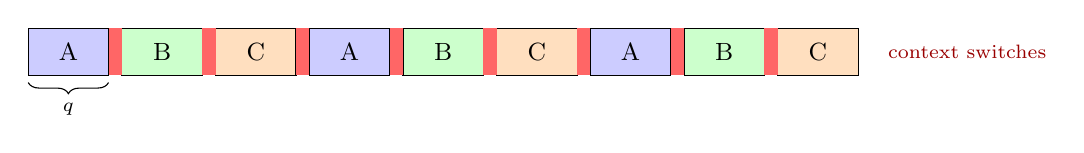
\begin{tikzpicture}[x=0.85cm, y=0.6cm, font=\small]
  \foreach \i/\n/\c in {0/A/blue!20, 1/B/green!20, 2/C/orange!25, 3/A/blue!20, 4/B/green!20, 5/C/orange!25, 6/A/blue!20, 7/B/green!20, 8/C/orange!25}
    \draw[fill=\c] (\i*1.4,0) rectangle node{\n} (\i*1.4+1.2,1);
  \foreach \i in {0,...,7} \fill[red!60] (\i*1.4+1.2,0) rectangle (\i*1.4+1.4,1);
  \draw[decorate, decoration={brace, amplitude=4pt, mirror}] (0,-0.15) -- (1.2,-0.15) node[midway, below=4pt, font=\scriptsize]{$q$};
  \node[font=\scriptsize, red!60!black, anchor=west] at (12.7,0.5) {context switches};
\end{tikzpicture}
\end{center}
Round robin with quantum $q$; each thin bar is a context switch, pure
overhead that grows relative to useful work as $q$ shrinks.

\section{Common pitfalls}
\begin{itemize}
  \item Assuming threads run in fork order --- they may run in any interleaving.
  \item Passing a pointer to a stack variable of the parent to a child thread, then returning
    from the parent function: the child now reads garbage.
  \item Confusing \code{thread\_yield} (stays runnable) with sleeping on a wait channel (needs
    a wakeup).
\end{itemize}

\section*{Summary}
\begin{itemize}
  \item A thread = PC + registers + stack; threads of a process share code, data and heap.
  \item A context switch saves the old thread's registers (OS/161: a \code{switchframe} on its
    stack), picks a new thread, and restores its registers.
  \item Threads are running, ready (ready queue) or blocked (wait channel).
  \item Preemption uses timer interrupts and a scheduling quantum to timeshare the CPU.
\end{itemize}
